% Setup
\documentclass[a4 paper, 12pt]{article}

% Title
\title{MEDIUM FIDELITY}

% Margins
\usepackage{geometry}
\geometry{margin=2cm}

% Images
\usepackage{graphicx}
\usepackage{float}
\usepackage[export]{adjustbox}
\setlength{\intextsep}{5pt plus 2pt minus 2pt}
\setlength\belowcaptionskip{0ex}
\usepackage[font=footnotesize,skip=2pt]{caption}

% Paragraph
\setlength{\parindent}{2em}
\setlength{\parskip}{1em}

% Text Formatting
\usepackage[utf8]{inputenc}
\usepackage[english]{babel}

% List spacing
\usepackage{enumitem}
\setlist{noitemsep, topsep=0pt}
\setlist[enumerate]{parsep=5pt} 

% Text Color
\usepackage{xcolor}

% Hyperlinks
\usepackage{hyperref}
\hypersetup{
    colorlinks=true,
    linkcolor=black,
    filecolor=black,      
    urlcolor=blue,
}

% Appendix
\usepackage{appendix}

% Include pdf
\usepackage{standalone}
\usepackage{pdfpages}

% Borders
\usepackage{mdframed}

% Symbols
\usepackage{amssymb}

\usepackage{multicol}
%%%%%%%%%%%%%%%%%%%%%%%%%%%%%%%%%%%%%%%%%%
\begin{document}

\section{Medium Fidelity Prototype}
The medium fidelity prototype is the first digital version of the application. It follows the research and initial conceptual design of the low fidelity prototype, while revising these concepts using the analysis of the first round of evaluations. The main sections of misunderstanding are from restaurant to comparison list, and comparison list to restaurant. To better understand the users and the usability of the app, this section additionally includes personas, scenarios and UX Goals. 

\subsection{Revised Requirements/Conception Design}
From the low fidelity evaluations the initial requirements and conceptual designs will be revised accordingly. This includes more detail to the design principles and system requirements. 

    \subsubsection*{System Concept Statement}
    The problem statement and high-level description of the outlined in the low fidelity prototype are still accurate for the next iteration, as well as the definition of mobile paradigm and instructing mode. However, whilst most of the metaphors were accurately chosen, there were several that either didn't align with the user's mental models or the defined design principles. 
    
    The following updated metaphors will be applied to this next iteration.
        \begin{itemize}
            \item Explore: map with location marker $\dashrightarrow$ compass
            \item List: bookmark $\dashrightarrow$ scales
            \item Deals: coupon $\dashrightarrow$ offer
        \end{itemize}

    \subsubsection*{Design Principles}
    The design principles were briefly identified for the low fidelity prototype. With the feedback from the user evaluations, more substantial detail of how to achieve these goals, as well as the addition of new principles are introduced. There are three additional design principles:
        \begin{multicols}{3}
            \begin{itemize}
                \item Minimal Effort
                \item Purposeful movement
                \item Consistency
            \end{itemize}
        \end{multicols}
    In order to satisfy these principles and those previously stated, the below will be taken into consideration for the prototype.
    \begin{multicols}{2}
        \begin{itemize}
            \item Colour
                \begin{itemize}
                    \item Common color schemes (red error)
                    \item Consistent colour throughout
                    \item Follow recognizable colour schemes
                    \item Hierarchical visuals (colour, text)
                \end{itemize}
            \item Font
                \begin{itemize}
                    \item Use popular font
                    \item Avoid jargon
                \end{itemize}
            \item Graphics
                \begin{itemize}
                    \item Use industry standards metaphors                            
                    \item Standard mapping display 
                \end{itemize}    
            \item Gestures
                \begin{itemize}
                    \item Standard gestures (swipe, zoom)
                \end{itemize}
            
            \item Dropdowns - Proximity
                \begin{itemize}
                    \item Dropdown/hidden menus
                \end{itemize}
             
            \item Navigation tabs - continuity
                \begin{itemize}
                    \item Navigation tabs top and bottom
                    \item Navigation bars consistent and locked
                    \item Highlight active interfaces 
                \end{itemize}
            \item Hicks Law - choosing right number of choices
                \begin{itemize}
                    \item Minimise user input
                    \item Keep interface elements to a minimum
                    \item Don't overload with options
                \end{itemize}
            \item Fitts law - large buttons, keep things close
                \begin{itemize}
                    \item Less movement between pages
                    \item Large actionable buttons 
                \end{itemize}
            \end{itemize}
        \end{multicols}     
    


        % \begin{multicols}{2}
        %     \begin{itemize}
        %         \item Give clear direction and guidance
        %             \begin{itemize}
        %                 \item make actions clearer
        %                 \item push users behaviour
        %                 \item Common color schemes (red error)
        %                 \item Minimise user input
        %                 \item Highlight active interfaces
        %                 \item Hierarchical visuals (colour, text)
        %                 \item Navigation bars consistent and locked
        %             \end{itemize}
        %         \item Be familiar
        %             \begin{itemize}
        %                 \item Use industry standards metaphors
        %                 \item Use popular font
        %                 \item Follow recognizable colour schemes
        %                 \item Standard gestures (swipe, zoom)
        %                 \item Standard mapping display
        %                 \item Common color schemes (red error)
        %                 \item Avoid jargon
        %             \end{itemize}
        %         \item Simplify decision process
        %             \begin{itemize}
        %                 \item Move less between pages
        %                 \item Actionable buttons
        %                 \item Keep interface elements to a minimum
        %             \end{itemize}
        %         \item Encourage collaboration
        %             \begin{itemize}
        %                 \item Make clear there are friend recommendations
        %             \end{itemize} 
        %         \item Maximise customisation opportunities
        %             \begin{itemize}
        %                 \item Minimise user input
        %                 \item Dropdown/hidden menus
        %                 \item Keep interface elements to a minimum
        %                 \item Don't overload with options (Hicks Law)
        %             \end{itemize}
        %         \item Open to change 
        %             \begin{itemize}
        %                 \item 
        %             \end{itemize}
        %         \item Manageable steps
        %             \begin{itemize}
        %                 \item Navigation tabs top and bottom
        %                 \item Dropdown/hidden menus
        %                 \item Don't overload with options (Hicks Law)
        %                 \item Keep interface elements to a minimum
        %                 \item Minimise user input
        %             \end{itemize}
        %         \item [$\circledcirc$] Minimal Effort
        %             \begin{itemize}
        %                 \item Popular metaphors
        %                 \item Clear actions
        %                 \item Less movement between pages
        %                 \item Standard mapping display
        %                 \item Avoid jargon
        %                 \item Keep interface elements to a minimum
        %                 \item Minimise user input
        %             \end{itemize}
        %         \item [$\circledcirc$] Purposeful movement
        %             \begin{itemize}
        %                 \item have actions available without going to another page
        %                 \item minimise movement on page to perform action
        %                 \item Standard gestures (swipe, zoom)
        %                 \item Informative motion
        %             \end{itemize}
        %         \item [$\circledcirc$] Consistency
        %             \begin{itemize}
        %                 \item Navigation bars consistent and locked
        %                 \item popular metaphors
        %                 \item popular fonts
        %                 \item same colour throughout
        %                 \item Hierarchical visuals (colour, text)
        %             \end{itemize}  
        %         \end{itemize}
        %     \end{multicols}
        



            
              
   




    \subsubsection*{System Requirements}


        -- Add profile page
        -- Make it clear that the shareable list is an option, update to a comparison rather than a list (confusing with favourite list)
        -- Make clear that everything is filtered - this was important but not obvious
        -- Recommend to everyone not just friends
        -- Users want easier access to the information in more places


        - Dropdowns - Proximity
        - Navigation tabs - continuity
        
        - Hicks Law - choosing right number of choices
        - Fitts law - large buttons, keep things close
        - design patterns - 
        - consistent inferface



\subsection{Personas}
To summarise and empathize with the users of the system, four personas have been developed. Each of these personas represent a different type of user to provide an overview of each group's expectations, use cases and highlight the most important functionality they need (Yale, 2020; usability.gov, 2020). There is a typical user as well as one at each end of the extremes (low and high use) and a user who requires the use of less required elements (dietary and planning). Each persona has a name, photo, life goal, blurb, quote relating to the system and an overview of their characters (employment, relationship status, income, interests, use of the system, restrictions). The full breakdown of each persona can be viewed in Appendix B.1.
    \begin{figure} [H]
        \centering
        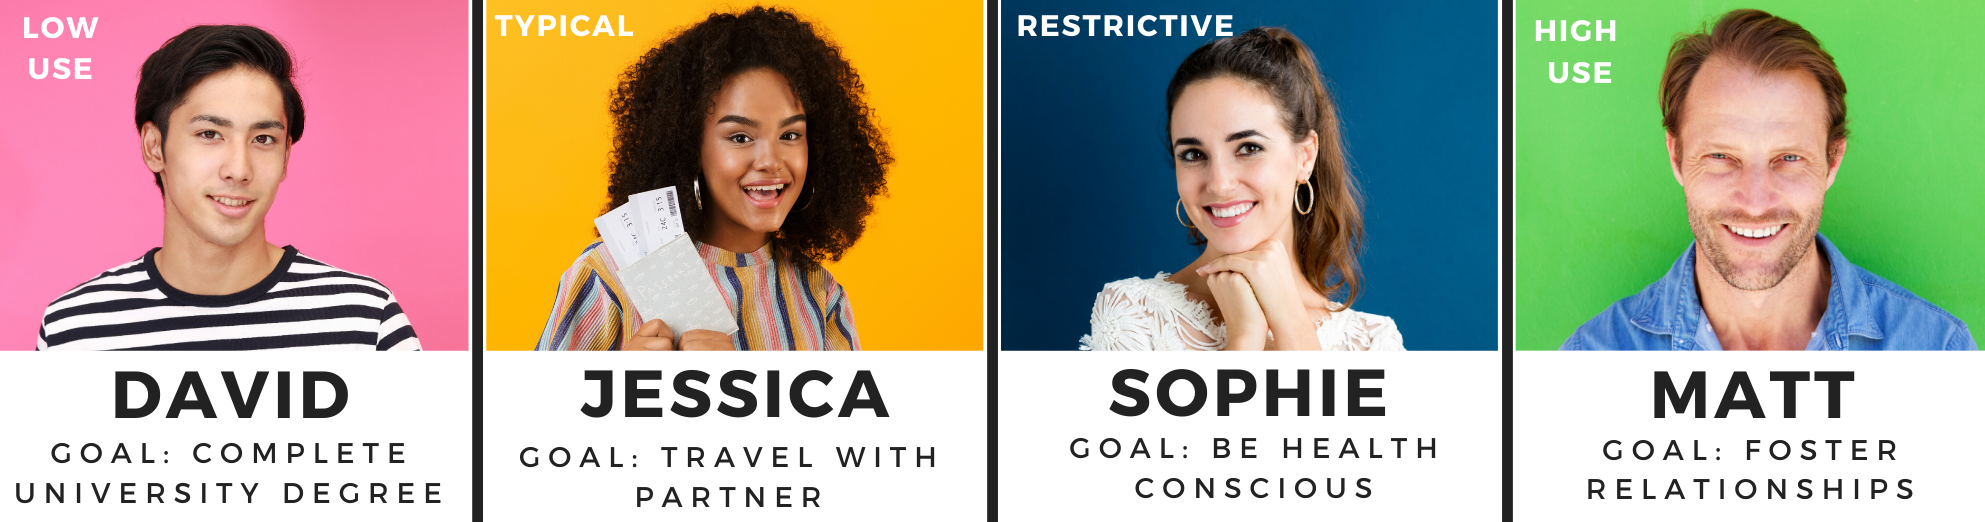
\includegraphics[width=\textwidth, frame]
            {./images/personas_overview.PNG}
        \caption{Personas Overview}
    \end{figure}  


\subsection{Interaction Scenarios}
For each of the created persona's a storyboard of their typical interaction with the system was sketched. These scenarios communicate the subsets of user behaviour of the system to assist with ensuring all users needs are met and that the design of the system supports these expectations. Each scenario has 11 slides and uses the template supplied by NNGroup with rough sketches and simple explanations. There are four scenarios, all of which can be found in Appendix B.2.
    \begin{enumerate}
        \item David - Student Deals - Find the cheapest place with friends
        \item Jessica - Hump Day - Choose from favourites with partner
        \item Sophie - Busy Planner - Plan lunch ahead
        \item Matt - Lunch at work - Choose first nearby, recommended place
    \end{enumerate}


\subsection{UX Goals}
When determining the 'success' of the user experience it is important to 'focus on the outcome not the feature' (NNGroup). Rather than focus on the service the application is offering, focus on the problem that this application is solving. The problem is that no existing solutions that give users what they actually want (the benefits); options to dine out with others based on personal preference (craving, dietary), nearby location and word-of-mouth recommendations.

These UX Goals were developed by identifying the main user needs, from previous evaluations and research, and then selecting content and functionality requirements to meet them. The goals use SMART principles and together cover all systems requirements. Each goal is a real-world end state that users want to reach (Yale, 2020). The full details of the UX goals can be found in Appendix B.3, including their source, measures and link to requirements.
    \begin{enumerate}
        \item I want to dine out at places that match my dietary requirement.
        \item I want to eat what I am craving.
        \item I want to choose where to eat based on my location.
        \item I want to view the menu of the restaurant as it relates to me before going there.
        \item I want to learn about the relevant deals of a restaurant.
        \item I want access to the basic information of a restaurant.
        \item I want to compare a variety of restaurants at once.
        \item I want to share the experience of dining out with friends.
        \item I want to dine out at restaurants that have been recommended by word-of-mouth.
        \item I want to re-visit restaurants that I enjoyed.
        \item I want to find new places to eat out.
        \item I want to dine out in my budget.
        \item I want to decide where to dine out in less than 20 minutes.
        \item I want support restaurants without having to leave long reviews.
    \end{enumerate}

\subsection{Prototype Development}
Taking into consideration the revised requirements as outlined from the results of the low fidelity prototype evaluations a medium fidelity prototype was created. Figma was chosen due to its browser-based interface, easy-to-use design, prototype functionality and popularity in the UX world. Colour, icons and basic functionality has been implemented. Since this is the first digital version of the prototype, the same interaction as the low fidelity prototype was implemented (only one end option for each feature). 

In addition to the updates on the pages of the low fidelity prototype, the following design choices were made to follow the well documented industry standards outlined by material design to align with several of the design principles; be familiar and minimal effort. These standards are not only thoroughly researched to ensure the optimal user experience, but their popularity creates a sense of familiarity for users which greatly reduces cognitive load (especially in terms of memory, learning, and pattern and recognition). 
    \begin{itemize}
        \item The appearance of the icons is in-line with material design where possible. Some of these icons take advantage of closure in gestalt's theory (users complete borders themselves). The only icon that had to be sourced elsewhere was the scales for the compare feature.        
            \begin{figure} [H]
                \centering
                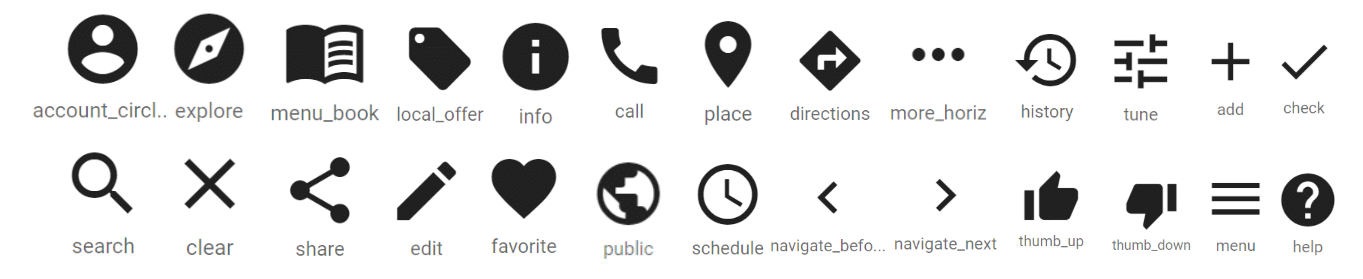
\includegraphics[width=\textwidth, frame]
                    {./images/material_icons.PNG}
                \caption{Icons - Material Design}
            \end{figure}                 
        \item The primary colour, used for a majority of the application, is 'medium violet red'. This colour was selected as pink is calming, joyful and encourages creativity (Cherry, 2019, which aligns with the aim of wanting to users to enjoy the experience of choosing where to dine out. Variants of the primary colour are used in contrast to distinguish different elements and were chosen using the palette generator from materialdesign.io. The light variant is 'lavender blush' and is used to fill buttons when they are selected. This follows a monochromatic scheme which produces a soothing effect and is easy on the eyes (). By using specific colours this also assists with reducing cognitive overload using gestalts theory of similarity.
            \begin{figure} [H]
                \centering
                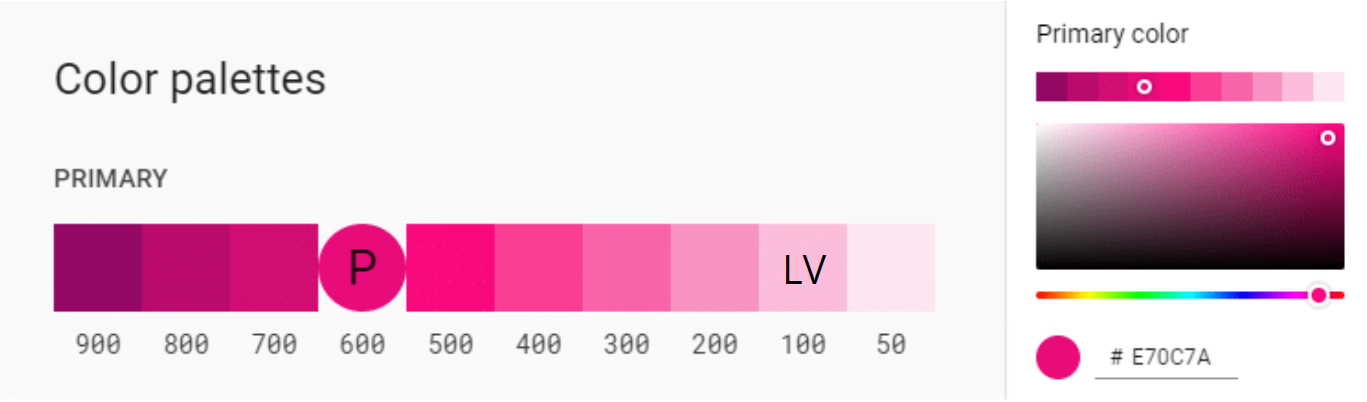
\includegraphics[width=0.8\textwidth, frame]
                    {./images/colour_med.PNG}
                \caption{Colour Palette - Medium Violet Red}
            \end{figure}
        \item The only font used throughout the app is 'roboto'. It is the default font for Android and many Google services (Jackson, 2020). The colour of the font is either the primary, white or grey depending on the background.
            \begin{figure} [H]
                \centering
                
\includegraphics[width=0.8\textwidth, frame]
                    {./images/font.PNG}
                \caption{Font - Roboto}
            \end{figure}
        \item The application now has a name; foodie. It is simple and fun. It will replace APPNANE in the top navigation bar. 
    \end{itemize}





The below is the interface of the medium fidelity prototype, with any relevant updates outlined. 
    \begin{figure} [H]
        \centering
        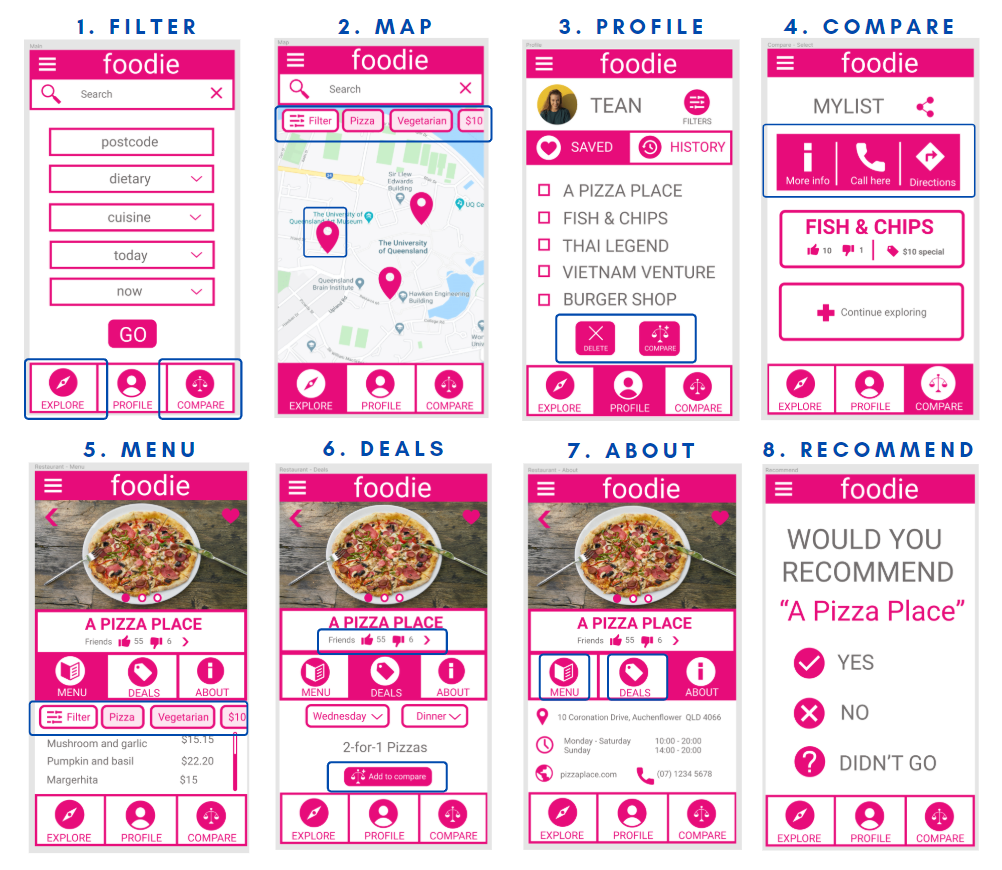
\includegraphics[width=\textwidth, frame]
            {./images/med_prototype.PNG}
        \caption{Medium Prototype}
    \end{figure}   

\begin{enumerate}
    \item Filter - Change the name for LIST to COMPARE. Update EXPLORE to the more recognised metaphor of a compass and the COMPARE symbol with scales.
    \item Map - Add shading to the selected filters. Update the circles for the places with the location marker.
    \item Profile - Frame selection icons as buttons for consistency.
    \item Compare - Remove selection icons from bottom and replace with overlay of more options when selected. 
    \item Menu - Add filter component from MAP page to show the menu is filtered.
    \item Deals - Add 'friends' label and option to navigate to see all recommendation reviews. Move 'add to list' icon to large button in the main area and update to match new list details.
    \item About - Use the icons from material design to represent MENU and OFFER. Also remove star reviews.
    \item Recommend - There are no changes from the low fidelity.
\end{enumerate}
 

\subsection{Evaluation Methods}
Instead of evaluating whether the application assists users with solving a problem the purpose of the evaluations of the medium fidelity is to determine the usability of the application. Any gaps between mental models in the low fidelity prototype have been amended for the medium fidelity prototype and it has been determined that this application is something users want, so now its a matter of whether they can use it.  

The think aloud evaluation method requires users to either complete a specific task or walk through all aspects of the application, whilst saying out loud everything they are thinking. This method was chosen as it provides substantial qualitative feedback on the user's experience as it is happening in regards to their expectations of the system. Since the end goal for this application is the same for every user, deciding where to dine out, the process of deciding is different for every user with a wide range of approaches that can be taken with the system.

The System Usability Scale (SUS) is a set of 10 questions, with both positive and negative responses, that provides a grade for the usability of the system. These questions are a popular staple of evaluation in the user experience industry as they are are cheap and quick process. Since the user is only required to respond with a numerical value, the full picture of why and how users feel about a system may be missing. This is used to supplement the think aloud evaluation as it provides an overall quantitative picture of the user experience after an overload of qualitative feedback.


\subsection{Evaluation Protocol}
The purpose of this protocol, structure and consistency, is the same as the low fidelity prototype. The protocol can be viewed in Appendix B.1. Also similarly, users are invited to a Google Form where all instructions, links and surveys are available to them. The form can be viewed in Appendix B.2. After providing consent the user will be directed to an interactive prototype. Each page of the prototype in presentation is outlined by a typical android smartphone frame. The slides can be viewed in Appendix B.6. 

Users are asked to use the app as if they were a first time user interested in the app. They are given no specific task and to speak all thoughts out loud. This is inline with the Think Aloud evaluation method. In addition to taking note of their use and understanding of components of the prototype, the measures for the UX goals will also be taken simultaneously. After explaining each step of the system as they understand, users will be directed back to the Google Forms to complete the SUS questionnaire. 

\subsection{Evaluation Results}
The following provides an overview of the results and feedback from the evaluations and is separated by the key features of the application.

\begin{enumerate}
    \item Filter by preferences (including both craving and dietary requirements) - this filtering extends to the map results and menu display
        \begin{itemize}
            \item 
        \end{itemize}

    \item Interactive map - replicate the familiar experience of exploring destinations
        \begin{itemize}
            \item 
        \end{itemize}

    \item Promote existing deals - have existing deals from restaurants separate from the menu and easily viewable based on date selection
        \begin{itemize}
            \item 
        \end{itemize}

    \item Editable and shareable list - provide support to be able to compare options and share these with others
        \begin{itemize}             
            \item 
        \end{itemize}

    \item Recommend to a friend - focus on word-of-mouth recommendations instead of star ratings
        \begin{itemize}
            \item 
        \end{itemize}

    \item Restaurant information - ensure users are able to readily access general information about a restaurant without being overwhelmed 
        \begin{itemize} 
            \item   
        \end{itemize}
\end{enumerate}


\subsection{Evaluation Analysis}









\end{document}